\documentclass{standalone}
\usepackage{tikz}
\usepackage{ctex,siunitx}
\usepackage{tkz-euclide}
\usepackage{amsmath}
\usetikzlibrary{patterns, calc}
\usetikzlibrary {decorations.pathmorphing, decorations.pathreplacing, decorations.shapes,}
\begin{document}
\small
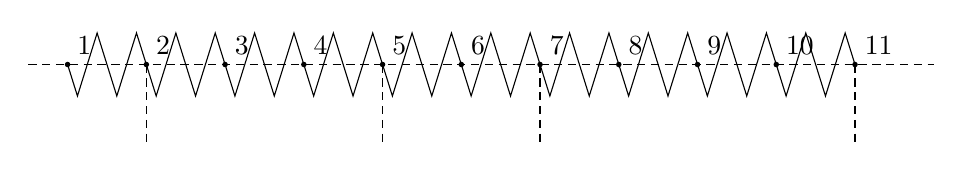
\begin{tikzpicture}[>=stealth, scale=1.0]
  \draw [densely dashed](-0.5,0)--(11,0);
  \foreach \x[ count=\i] in {0,1,...,9}
  {
    \fill(\x,0)circle(1pt)node[above right]{\i};
    \draw(\x,0)--++(0.125,-0.4)--++(0.25,0.8)--++(0.25,-0.8)--++(0.25,0.8)--++(0.125,-0.4);
  }
  \fill(10,0)circle(1pt)node[above right]{11};
  \foreach \x in {1,4,6,10 }{ \draw[thin,densely dashed] (\x,0)--(\x,-1.0);}
\end{tikzpicture}
\end{document}